\documentclass{article}
\author{Jake Kolevas, Aidan Gresko}
\title{Main Simulator}
\date{\today}

\usepackage{times}
\usepackage{tcolorbox}
\usepackage{graphicx}
\usepackage{float}
\usepackage{amsmath}
\usepackage{siunitx}

\begin{document}
	\maketitle
	
	\section{Overview}
	This project involves writing a base power systems modeling package in Python. The code establishes basic classes for the main power system components – buses, generators, conductors, geometries, and an overarching Circuit class to link them. The Circuit class facilitates the establishment of a network, calculation of significant values like equivalent distance between conductors, and lastly, the construction of the network admittance matrix (Y-bus) – a critical step towards load flow analysis and power system study. The code offers a modular environment available for parallel development and, therefore, future expansion to include additional components, advanced modeling capabilities, and perhaps integration with other power system analysis software programs. The objective is to provide a flexible and customized platform for discussing power system concepts and performing basic analysis.
	
	\section{Class Diagram}
	
	\begin{figure}[H]
		\centering
		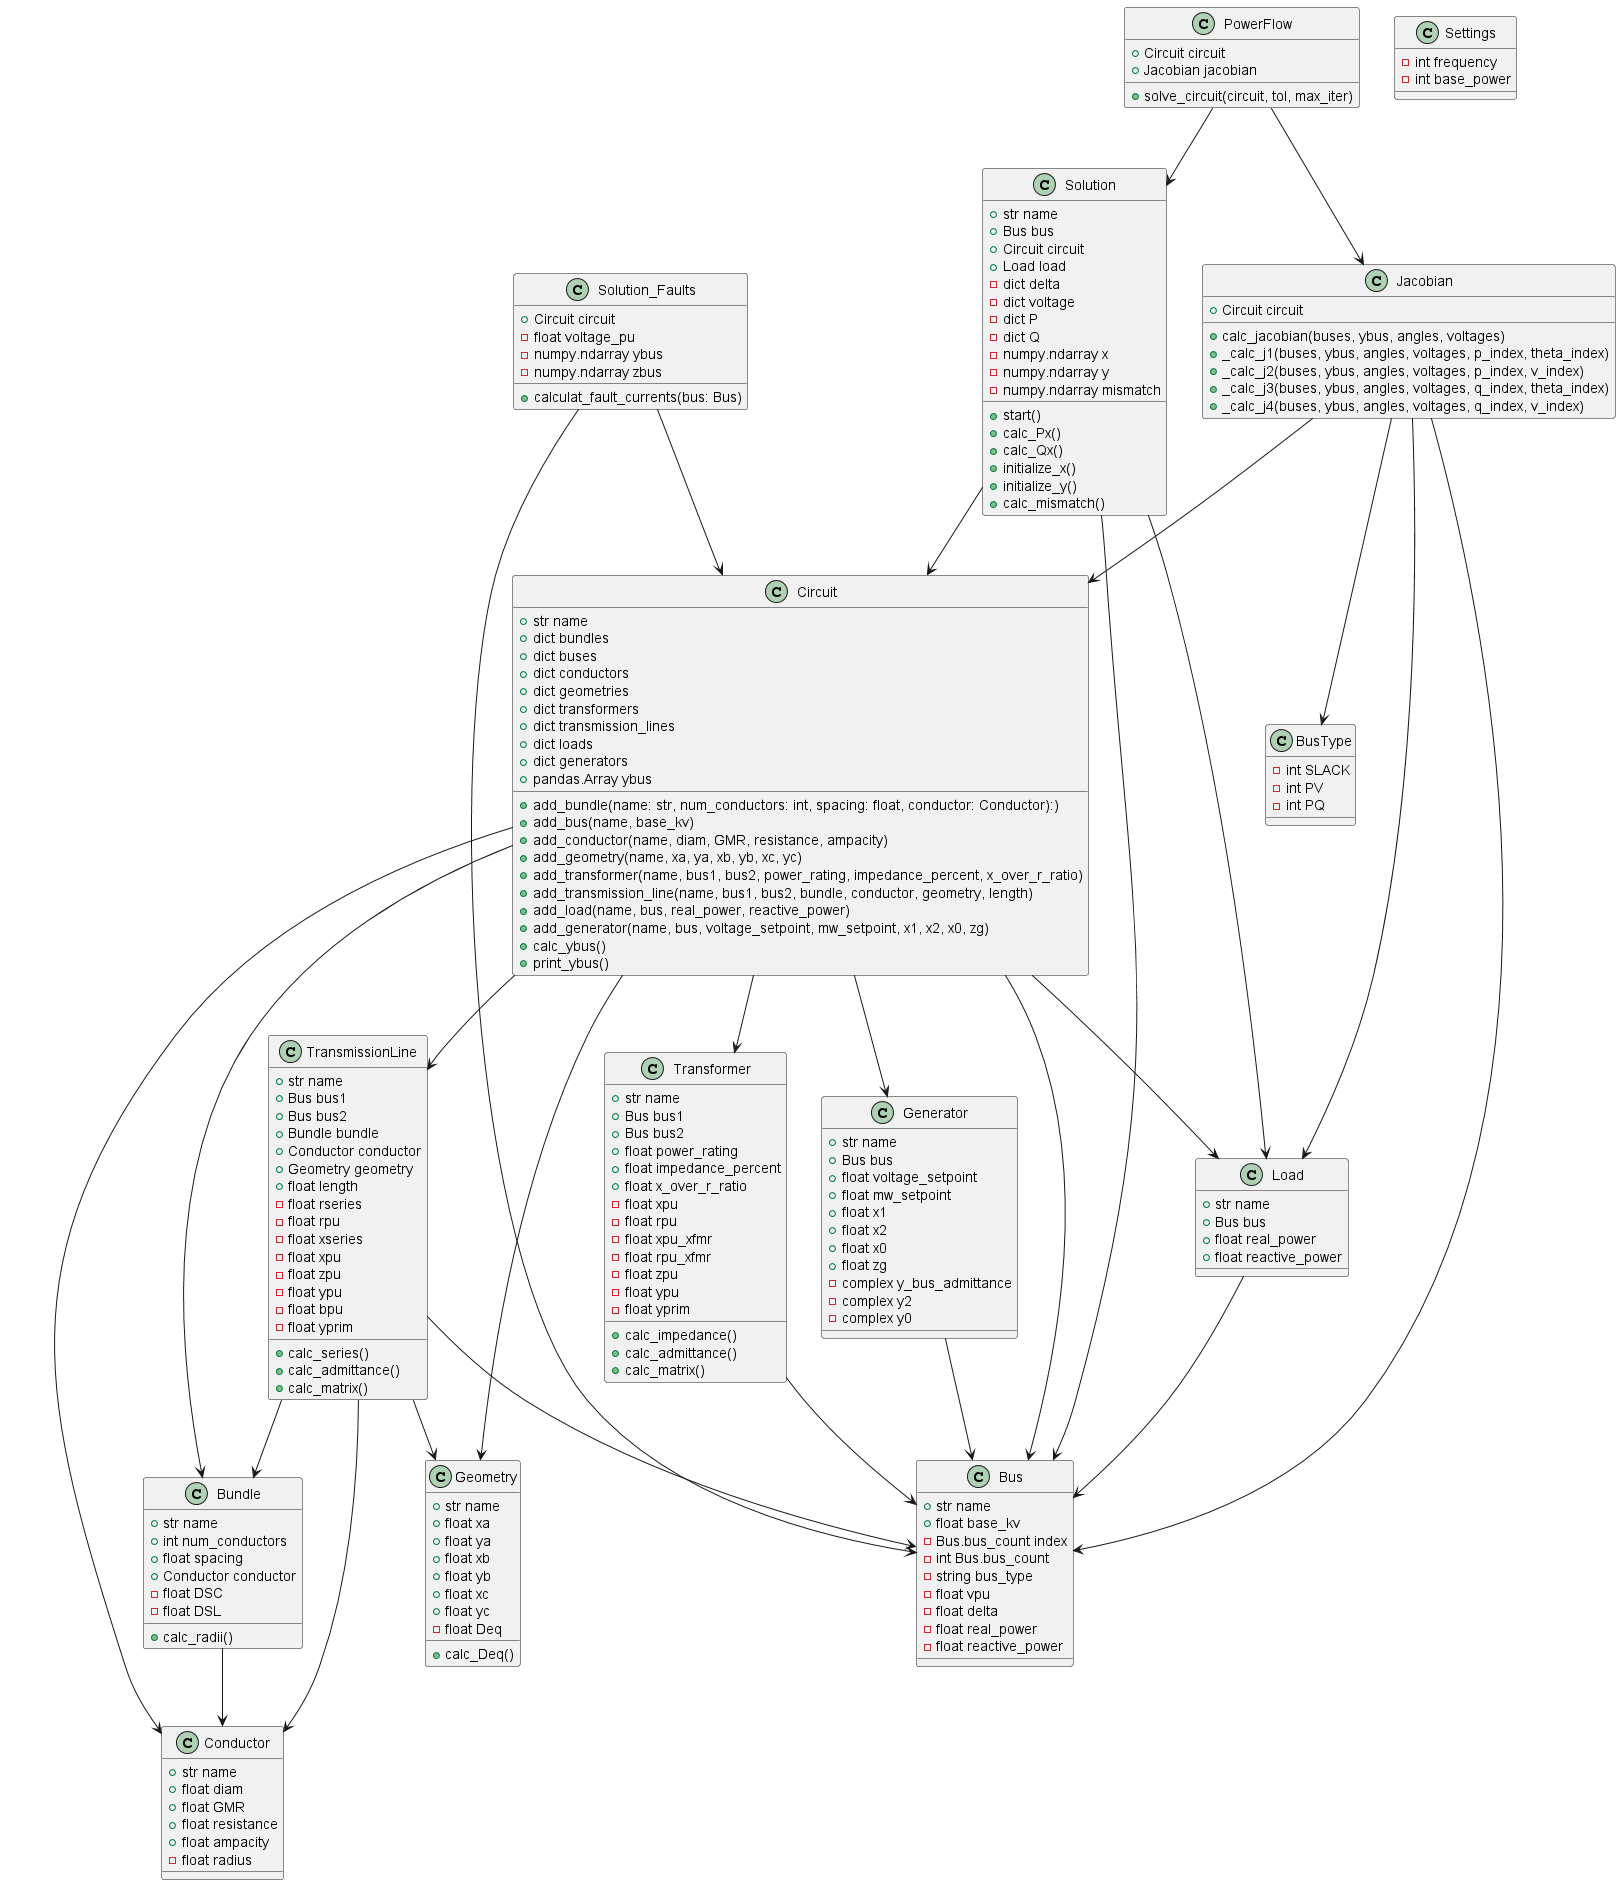
\includegraphics[scale=0.25]{../out/circuit/circuit.png}	
		\caption{Class Diagram for Project}
	\end{figure}
	
	\section{Classes}
	
	\subsection{Bundle}
	The Bundle class models a collection of conductors used in this simulation and calculates effective radii for resistance and inductance computations. This class is essential for modeling transmission lines, as it helps accurately compute effective radii for conductors arranged in bundles, affecting overall line behavior in analyses.
	
	\subsection{Bus}
	This Bus class is designed to model various types of buses within the power system, such as Slack, PV, and PQ buses. Each Bus instance is initialized with a name and base voltage (base\_kv). The class maintains a count of all Bus instances created using the class-level variable bus\_count. Key attributes include the bus type, voltage per unit (vpu), phase angle (delta), and power values (real\_power and reactive\_power). This class serves as a foundational component for simulating and analyzing power systems, enabling tracking of essential electrical characteristics for each bus.
	
	\subsection{Circuit}
	The Circuit class serves as a foundational component for modeling this power systems. It encapsulates the various elements that comprise a circuit—including buses, conductors, bundles, transformers, transmission lines, loads, and generators—providing a structured framework for representing and analyzing power flow. The class allows users to define and connect these components, storing their properties and relationships.  A key functionality is the calc\_ybus method, which computes the network admittance matrix (Y-bus) which is crucial for power system analysis. This class forms the basis for more complex power system studies, enabling simulations of load flow, fault analysis, and system stability.
	
	\subsection{Conductor}
	The Conductor class is designed to model electrical conductors by initializing them with key properties such as name, diameter (diam), geometric mean radius (GMR), resistance, and ampacity. Upon instantiation, these parameters are assigned to instance variables, and the radius is calculated by converting the diameter from a given unit to inches using a divisor of 24.
	
	\subsection{Generator}
	The Generator class models a generator component within this  power system. Each generator is initialized with a name for identification, an associated bus reference (Bus), a target voltage level (voltage\_setpoint), and a target power output in megawatts (mw\_setpoint).
	
	\subsection{Geometry}
	The Geometry class models a geometric figure defined by three points (A, B, and C) with their respective coordinates. Upon initialization, it calculates an attribute Deq, which is the average distance between each pair of these points. This is achieved using the distance formula to compute the lengths of sides AB, BC, and AC, then averaging them. The class is useful for scenarios requiring a measure of the average side length of a triangle formed by three points.
	
	\subsection{Jacobian}
	The Jacobian class performs the Jacobian matrix calculation for power flow analysis in power systems. It provides methods for calculating each of the four submatrices (J1, J2, J3, J4) that constitute the total Jacobian. These include the real power (P) and reactive power (Q) sensitivities due to variations in voltage angles ($\delta$) and voltage magnitudes (V). The class crosses the network buses, computing these sensitivities from the admittance matrix (Ybus) and voltage angle and magnitude current estimates. The calculated Jacobian is a critical input to iterative power flow solvers, including the Newton-Raphson solution, to determine power system operating conditions. The functions within this class calculate efficiently the partial derivatives utilized for power flow convergence.
	
	\subsection{Load}
	The Load class is an electrical load that is connected to some bus in the power system. Each load is described by a name, a pointer to the `Bus` that it is connected to, and its real\_power and reactive\_power demands (in Watts and VARs, respectively). This class simulates the action of power usage at a node in the network and is a key object to be utilized within power system simulation and analysis. It allows demand modeling of the electricity grid and must be done in order to conduct load flow, contingency, and other power calculations.
	
	\subsection{Powerflow}
	The PowerFlow class computes the voltage magnitudes and angles of every bus in a power system circuit through the Newton-Raphson power flow algorithm. It is initialized with a circuit object that defines the network topology and parameters, and the power flow solution is determined iteratively. The solve\_circuit method performs the primary power flow calculation with a tolerance (tol) and maximum iterations (max\_iter). It employs a Jacobian object to calculate the Jacobian matrix and then proceeds to use it to update bus voltage angles and magnitudes iteratively until a converged solution is reached. The function returns a dictionary containing the convergence status, number of iterations, final mismatch, calculated voltage magnitudes and angles, calculated real and reactive power injections, and a history of the mismatch values during the iteration process, providing a complete overview of the power flow solution.
	
	\subsection{Settings}
	The Settings class is a store of global parameters used throughout the power system analysis. It currently sets the system frequency (in Hertz) and base\_power (in MVA), base values used for per-unit calculation and conversion. This class provides simple modification and consistent application of these essential system parameters, with the benefit of code maintainability and the flexibility to represent different power system configurations. While presently constrained, it is designed to be extensible with more global settings as needed.
	
	\subsection{Seven Bus Power System}
	This Seven Bus Power System illustrates the development and solution of a power flow study on a typical electrical power system. It outlines the creation of a network model, including bus data, line data, and load data, in a Python setting. The code calculates the Jacobian matrix, a critical component of the power flow equations' solution, and utilizes a Newton-Raphson method to determine bus voltages and power injections. Additionally, the Seven Bus incorporates fault analysis capability, calculating fault currents and determining bus voltages under fault conditions. The code forms a foundation for power system behavior simulation, network stability verification, and contingency analysis, ultimately demonstrating an integrated approach to power system modeling and analysis.
	
	\subsection{Solution}
	This Solution class implements a Newton-Raphson power flow solver for power system network analysis. It solves bus voltages by iterative minimization of the mismatch between calculated and specified power injections, utilizing an external `circuit` object to define network data and topology. The solver accommodates various bus types (Slack, PV, PQ) and features base MVA scaling for normalized calculations. By converging to a solution, it provides valuable information on steady-state operation, including voltage profiles and power flows, and is therefore a key building block for power system analysis.

	\subsection{Solution Symmetric}
	\dots	
	
	\subsection{Transformer}
	The Transformer class models transformers in a power system, connecting two buses and calculating their electrical characteristics like impedance and admittance. It's essential for simulating power flow and analyzing the system's behavior in this simulation.
	
	\subsection{Transmission Line}
	The TransmissionLine class encapsulates the electrical characteristics of a power transmission line. It initializes with necessary components such as buses, conductors, bundles, geometry, and length. The class computes series impedance (rpu, xpu) and shunt admittance (bpu) using given formulas. These values are then used to construct an admittance matrix (yprim), essential for power flow analysis. This model allows detailed simulation of how electrical power is transmitted between two points in a power system.
	
	\section{Equations Used for Power Calculations}

	\subsection*{Bundle}
	1 conductor: \\
	\begin{align*}
		& DSC = r \\
		& DSL = GMR (\text{geometric mean radius})
	\end{align*}

	\noindent	
	2 conductors: \\
	\begin{align*}
		& DSC = \sqrt{r * s} \text{ -- r is radius and s is spacing} \\
		& DSL = \sqrt{GMR * s}
	\end{align*}

	\noindent	
	3 conductors: \\
	\begin{align*}
		& DSC = \sqrt[n]{r * s^2} \\
		& DSL = \sqrt[n]{GMR * s^2}
	\end{align*}

	\noindent
	4 conductors: \\
	\begin{align*}
		& DSC = 1.091 * (r * s^4)^{1/4} \\
		& DSL = 1.091 * (GMR * s^4)^{1/4}
	\end{align*}
	
	\noindent
	Where: \\
	- DSC is the equivalent diameter of a single circular conductor \\
	- DSL is the geometric mean radius of the bundle \\
	- r is the radius of individual conductors \\
	- s is the spacing between conductors 
	
	\subsection*{Circuit}
	
	\begin{align*}
		& \text{Y-Bus}[i,i] = \text{sum of all self-admittances at bus i} \\
		& \text{Y-Bus}[i,j] = \text{-sum of mutual admittances between buses i and j} \\
		& Z_{\text{transformer}} = \frac{\text{base\_voltage}^2}{\text{power\_rating}} * \frac{\text{impedance\_percent}}{100} \\
		& G_{\text{line}} = \text{conductance per unit length} * \text{length} \\
		& B_{\text{line}} = \text{susceptance per unit length} * \text{length} \\
		& Z_{\text{line}} = R + jX
	\end{align*}
	
	\subsection*{Generator}
	
	\begin{align*}
		& Y_1 = 1/jX_1 \\
		& Y_2 = 1/jX_2 \\
		& Y_0 = 1/(jX_0 + 3Zg)
	\end{align*}
	
	\noindent
	Where: \\
	- Y represents admittance (per unit or Siemens) \\
	- X represents reactance (per unit or Ohms) \\
	- Zg represents ground resistance (Ohms) \\
	- j is the imaginary unit $(\sqrt{-1})$ 
	
	\subsection*{Geometry}
	Euclidean Distance Formula: $d = \sqrt{(x_2 - x_1)^2 + (y_2 - y_1)^2}$ \\
	
	\subsection*{Jacobian}
	Active Power: 
	\[
	P_i = V_i \sum_{j=1}^{n} V_j[G_{ij} \cos(\delta_i - \delta_j) + B_{ij} \sin(\delta_i - \delta_j)]
	\]
	
	\noindent
	Reactive Power: 
	\[
	Q_i = V_i \sum_{j=1}^{n} V_j[G_{ij} \sin(\delta_i - \delta_j) - \cos(\delta_i - \delta_j)]
	\]
	
	\noindent
	Jacobian Sub-matrices: \\
	
	\noindent
	J1: 
	\[
		J1_{ij} = 
		\begin{cases}
			\hfill -V_i^2 \sum_{k \neq i} Y_{ik} \sin (\delta_i - \delta_k - \theta_{ik}) \text{ if } i = j  \\
			\hfill V_i V_j Y_i \sin(\delta_i - \delta_j - \theta_{ik}) \text{ if } i \neq j
		\end{cases}
	\]
	
	\noindent
	J2:
	\[
		J2_{ij} = 
		\begin{cases}
			\hfill V_i Y_{ii} \cos(\delta_i - \delta_i - \theta_{ii}) + V_i \sum_{k \neq i} Y_{ik} \cos(\delta_i - \delta_k - \theta_{ik}) \text{ if } i = j \\
			\hfill V_i Y_{ij} \cos(\delta_i - \delta_j - \theta_{ij}) \text{ if } i \neq j
		\end{cases}
	\]
	
	\noindent
	J3: 
	\[
		J3_{ij} = 
		\begin{cases}
			\hfill V_i^2 \sum_{k \neq i} Y_{ik} \cos(\delta_i - \delta_k - \theta_{ik}) \text{ if } i = j \\
			\hfill -V_i V_j Y_{ij} \cos(\delta_i - \delta_j - \theta_{ij}) \text{ if } i \neq j
		\end{cases}
	\]
	
	\noindent
	J4: 
	\[
		J4_{ij} = 
		\begin{cases}
			\hfill -V_i Y_{ii} \sin(\delta_i - \delta_i - \theta_{ii}) + V_i \sum_{k \neq i} Y_{ik} \sin(\delta_i - \delta_k - \theta_{ik}) \text{ if } i = j \\
			\hfill V_i Y_{ij} \sin(\delta_i - \delta_j - \theta_{ij}) \text{ if } i \neq j
		\end{cases}
	\]
	
	\noindent
	Where: \\
	- $V_i$ and $V_j$: Voltage magnitudes at buses i and j \\
	- $G_{ij}$ and $B_{ij}$: Real and imaginary parts of the admittance between buses i and j \\
	- $Y_{ii}$: Admittance between buses i and j, where $Y_{ij} = G_{ij} + j B_{ij}$ \\
	- $\delta_i$ and $\delta_j$: Phase angles at buses i and j \\
	- $\theta_{ij}$: Phase angle of the admittance $Y_{ij}$
	
	\subsection*{PowerFlow}
	Newton-Raphson Method: 
	\[
	J \cdot dx = -\text{mismatch}
	\]
	
	\noindent
	Angle and Voltage Corrections: 
	\[
	\Delta \theta_{i}^{k+1} = \Delta \theta_i^k + dx_i
	\]
	
	\subsection*{Solution}
	Active Power Mismatch: 
	\[
	\Delta P_i = P_{spec,i} - P_i
	\]

	\noindent	
	Reactive Power Mistmatch: 
	\[
	\Delta Q_i = Q_{spec,i} - Q_i
	\]
	
	\subsection*{Solution Faults}
	Inverse Matrix: 
	\[
	Z_{bus} = (Y_{bus})^{-1}
	\]
	
	\noindent
	Fault Current at Bus: 
	\[
	I_f(n) = \frac{V_{pu}}{Z_{nn}}
	\]
	
	\noindent
	Bus Voltage Post-Fault: 
	\[
	V_k = (1 - \frac{ Z_{kn} }{ Z_{nn} }) \times V_{pu}
	\]
	
	\subsection*{Transformer}
	\noindent
	Transformer Impedance:
	\[ Z_{pu} = \frac{Z_\%}{100} \cdot \frac{S_{\text{base}}}{S_{\text{transformer}}} \angle{\theta} \]
	where \( \theta = \tan^{-1}(X/R) \). \\
	
	\noindent
	Transformer Admittance:
	\[ Y_{pu} = \frac{1}{Z_{pu}} \]
	
	\noindent
	Transformer Y-Bus Matrix:
	\[ [Y_{\text{Bus}}] = 
	\begin{bmatrix}
		Y_{11} & -Y_{12} \\
		-Y_{21} & Y_{22}
	\end{bmatrix} \]
	where \( -Y_{12} = -Y_{21} \).
	
	\subsection*{Transmission Line}
	Series Resistance Calculation: 
	\[
	R_{series} = (\frac{p}{n}) \times L
	\]
	
	\noindent	
	Series Reactance Calculation: 
	\[
	X_{series} = 2 \pi f \times \mu_0 \times \log(\frac{D_{eq}}{D_{SL}}) \times L
	\]
	
	\noindent
	Per Unit Impedance: 
	\[
	Z_{pu} = R_{pu} + j X_{pu}
	\]
	
	\noindent
	Shunt Admittance Calculation: 
	\[
	B_{shunt} = 2 \pi f \times \frac{\epsilon_0}{\log(\frac{D_{eq}}{D_{SC}})} \times L
	\]

	\noindent
	Per Unit Shunt Admittance Calculation: 
	\[
	B_{pu} = \frac{B_{shunt}}{Y_{base}}
	\]

	\noindent	
	Prim Matrix Calculation:
	\[
	Y' = \begin{bmatrix}
		Y_p + B/2 & -Y_p \\
		-Y_p & Y_p + B/2
	\end{bmatrix}
	\]
	
	\noindent
	Where: \\
	- \(Y_p\) is the per unit admittance due to series resistance and reactance. \\
	- \(B\) is the shunt conductance (real part of admittance).
	
	\section{Example Problem with Solution}
	
\end{document}
